\section{Theoretical Foundations}

  \subsection{Fundamentals of Semantic Segmentation}

    \subsubsection{Image Segmentation}

      \ti{Segmentation} is the process of breaking an image into groups of similar
      pixels\cite{intelligence2021modern}, dividing the image into segments. The
      goal of segmentation is to simplify the representation of an image into something
      that is more \ti{meaningful}, allowing more detailed analysis to be performed
      on each segment. There are two ways to approach the problem of segmentation:
      \ti{detecting boundaries} or \ti{detecting regions}\cite{intelligence2021modern}.

      \tb{Boundary detection} involves finding the boundaries between regions, using techniques
      such as edge detection with the Canny algorithm\cite{canny1986computational} or
      thresholding with the Otsu algorithm\cite{otsu1979threshold}. \tb{Region detection}
      involves finding regions of similar pixels, using techniques such as clustering
      with the K-means algorithm\cite{macqueen1965some} or the Mean-Shift algorithm\cite{comaniciu2002mean}.
      Figure \ref{fig:image_segmentation} shows an example of image segmentation using
      both boundary detection and region detection.

      \begin{figure}[htbp]
        \centering
        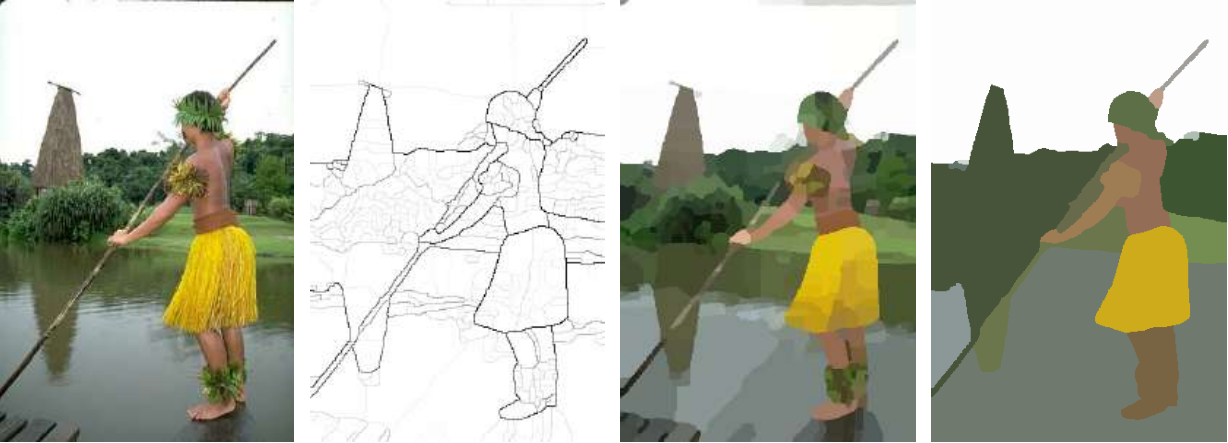
\includegraphics[width=1.00\linewidth]{theorical_foundations/image_segmentation.png}
        \caption{Image Segmentation using boundary and region detection \cite{intelligence2021modern}}
        \label{fig:image_segmentation}
      \end{figure}

    \subsection{Ground Truth}

      \ti{Ground Truth} in the context of semantic segmentation refers to the
      \ti{correct} segmentation of an image, manually annotated as segmentation masks
      that define the boundaries of the objects in the image\cite{intelligence2021modern}.
      The ground truth is used to train, validate and test semantic segmentation models. Pixel-level
      ground truth is the most common type of ground truth used in semantic segmentation
      datasets, where each pixel is assigned a label that defines the object it belongs.
      Figure \ref{fig:cityscapes_semantic_segmentation} and \ref{fig:kitti_semantic_segmentation}
      shows examples of pixel-level ground truth.
 
      \subsubsection{Cityscapes Dataset}

        \ti{Cityscapes} is a dataset for semantic urban scene understanding, containing
        $5000$ high quality pixel-level ground truth images, with $30$ classes of
        objects\cite{cordts2016cityscapes}. Figure \ref{fig:cityscapes_semantic_segmentation}
        shows an example of a Cityscapes image and its corresponding pixel-level ground truth.
        Dataset offers three different splits: \ti{train}, \ti{validation} and \ti{test}.
        As its used for numerous semantic segmentation models, it seems to be the most
        balanced dataset in terms of classes distribution. Also, having some hierarchy
        between classes, it is possible to group them into $8$ upper classes.

        \begin{figure}[htbp]
          \centering
          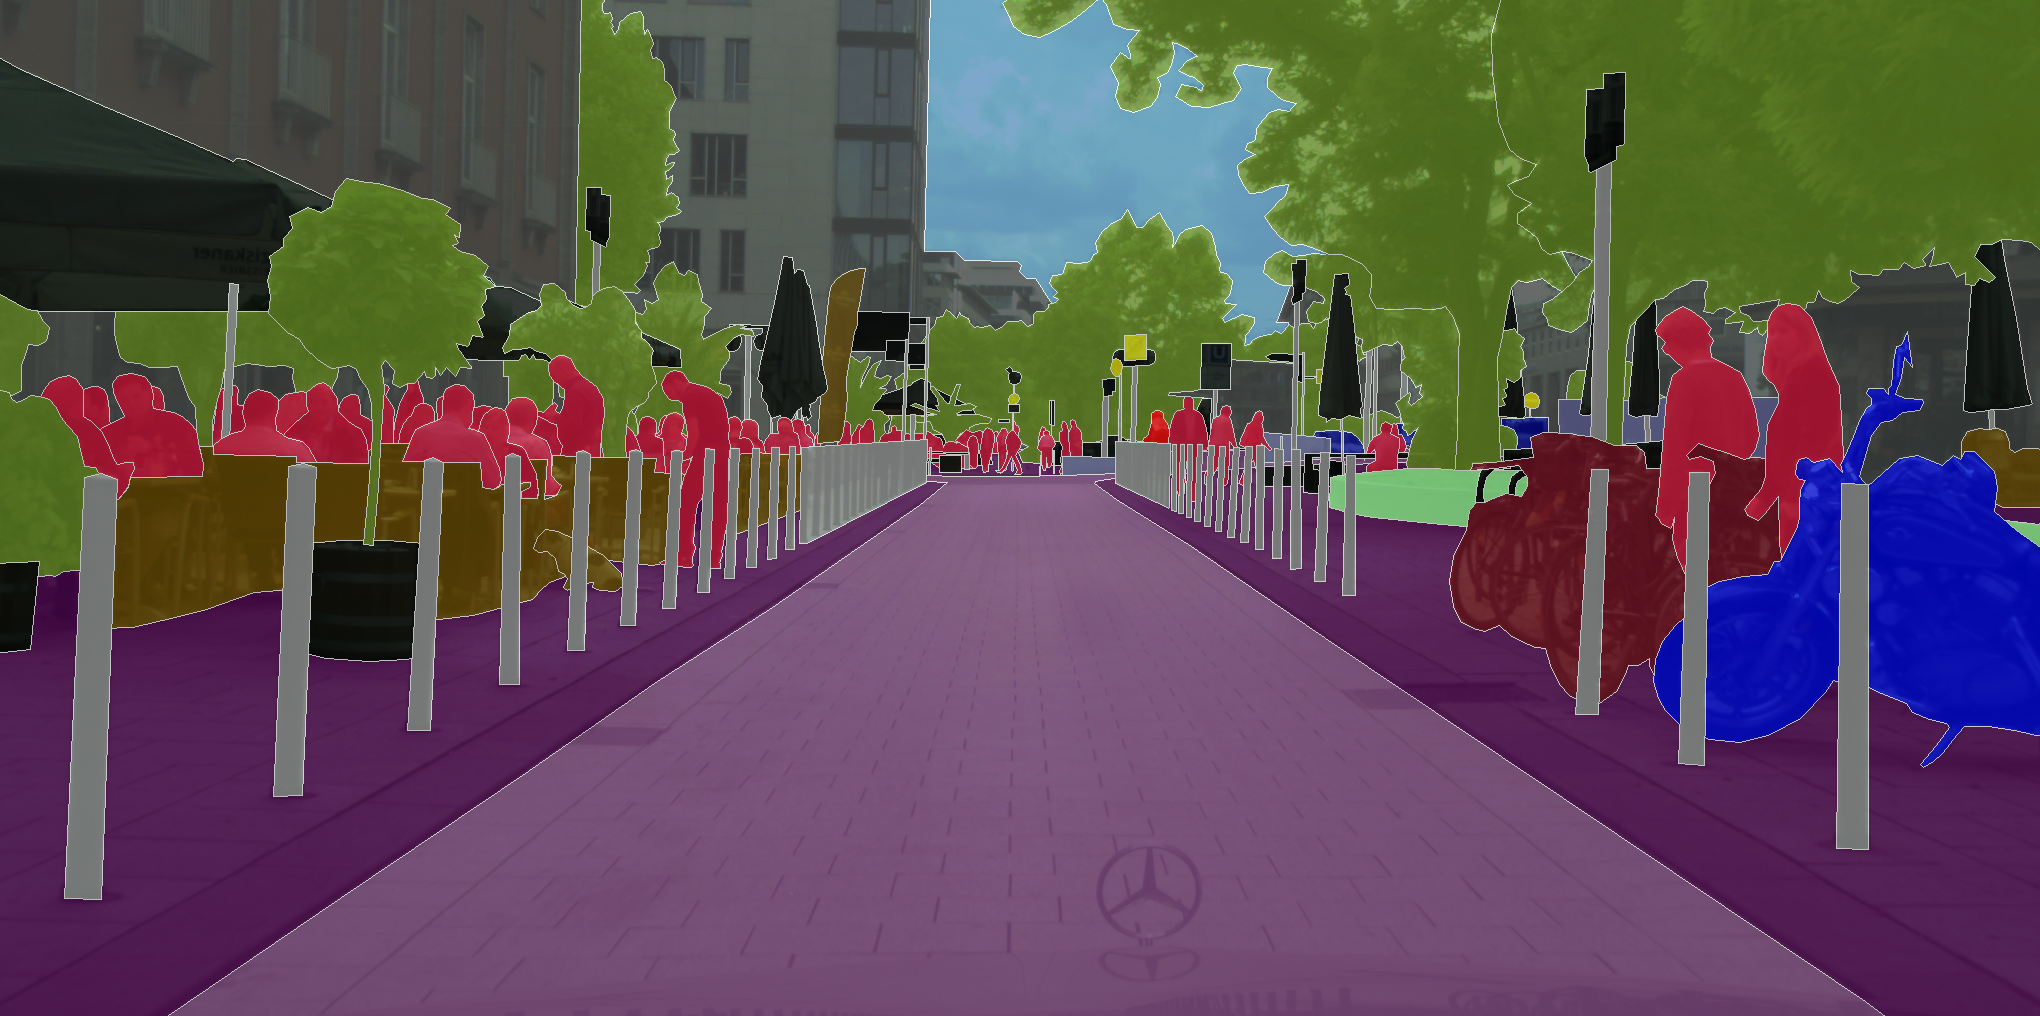
\includegraphics[width=1.00\linewidth]{theorical_foundations/cityscapes_stuttgart.png}
          \caption{Cityscapes semantic segmentation}
          \label{fig:cityscapes_semantic_segmentation}
        \end{figure}

      \subsubsection{KITTI Dataset}

        \ti{KITTI} is a dataset for autonomous driving, containing $200$ pixel-level
        ground truth images, with $34$ classes of objects\cite{Geiger2012CVPR}. Figure
        \ref{fig:kitti_semantic_segmentation} shows an example of a Kitti image and
        its corresponding pixel-level ground truth. Dataset offers two different splits:
        \ti{train} and \ti{test}. As its used for autonomous driving, it seems to be
        the most unbalanced dataset in terms of classes distribution. Also, having no
        hierarchy between classes, it is not possible to group them into upper classes.

        \begin{figure}[htbp]
          \centering
          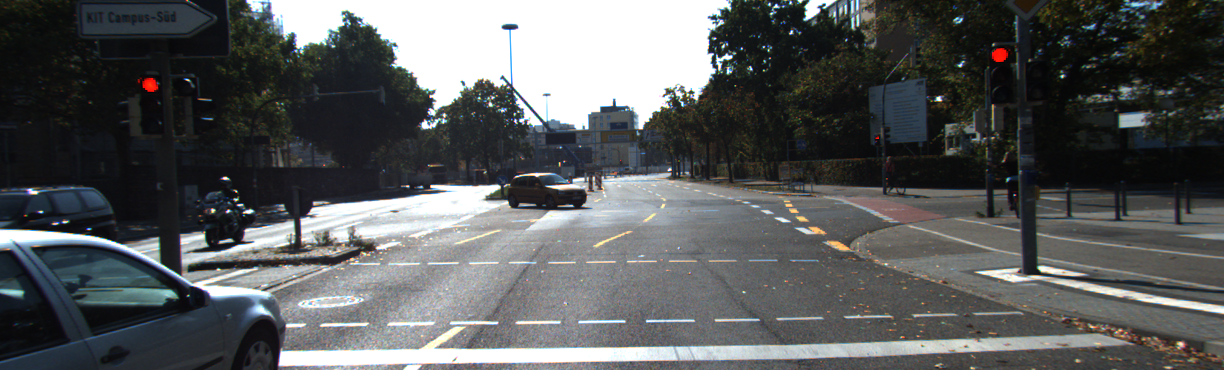
\includegraphics[width=1.00\linewidth]{theorical_foundations/kitti_000155.png}
          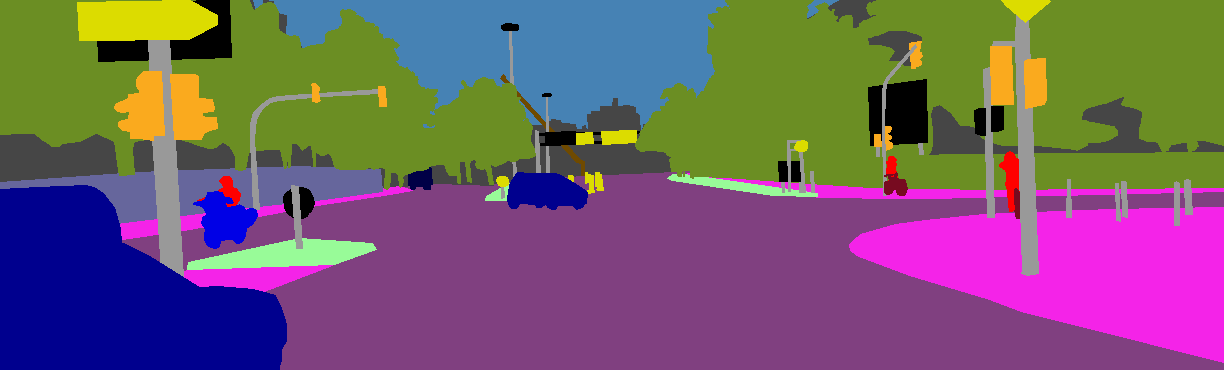
\includegraphics[width=1.00\linewidth]{theorical_foundations/kitti_000155_gt.png}
          \caption{Kitti semantic segmentation}
          \label{fig:kitti_semantic_segmentation}
        \end{figure}

  \subsection{Evaluation Metrics}

    \subsubsection{Pixel Accuracy}

      \ti{Pixel Accuracy (PA)} is the simplest metric used to evaluate the performance
      of a semantic segmentation model. It is calculated by cumputing the ratio
      between the number of correctly classified pixels and the total number of
      pixels in the image\cite{long2015fully}. The pixel accuracy is a value between
      $0$ and $1$, with $1$ being the best possible score.
      \begin{equation}
        \label{eq:pixel_accuracy}
        PA = \frac{TP_i + TN_i}{TP_i + TN_i + FP_i + FN_i}
      \end{equation}
      where $TP_i$ is the number of true positives (correct \ti{foreground pixels}),
      $TN_i$ is the number of true negatives (correct \ti{background pixels})
      meaning correctly classified pixels, $FP_i$ is the number of false positives
      (incorrect \ti{foreground pixels}) and $FN_i$ is the number of false negatives
      (incorrect \ti{background pixels}) meaning incorrectly classified pixels.

      Although the pixel accuracy is a simple metric, it is not a good metric to
      evaluate the performance of a semantic segmentation model. This is because
      the pixel accuracy does not take into account the \ti{class imbalance problem},
      presented in semantic segmentation datasets and real world scenarios.
      
    \subsubsection{Mean Pixel Accuracy}

      \ti{Mean Pixel Accuracy (mPA)} calculate the pixel accuracy(\ti{PA}) for each
      semantic category and then averages the results\cite{long2015fully}. The mPA is a value between $0$ and $1$,
      with $1$ being the best possible score.
      \begin{equation}
        \label{eq:mean_pixel_accuracy}
        mPA = \frac{1}{n} \sum_{i=1}^{n} PA_i
      \end{equation}
      using the same variables as in equation \ref{eq:pixel_accuracy} and $n$ is the
      number of semantic categories. However, the mPA still does not take into account
      the \ti{class imbalance problem}.

    \subsubsection{Intersection over Union}
      
      \ti{Intersection over Union (IoU)} or \ti{Jaccard index} is calculated by dividing
      the intersection of the predicted segmentation and the ground truth segmentation by the union
      of the predicted segmentation and the ground truth segmentation\cite{long2015fully}.
      The IoU is a value between $0$ and $1$, with $1$ being the best possible score.
      \begin{equation}
        \label{eq:iou}
        IoU = \frac{{|A \cap B|}}{{|A \cup B|}} = \frac{TP_i}{TP_i + FP_i + FN_i}
      \end{equation}
      where $A$ is the predicted segmentation, $B$ is the ground truth segmentation,
      $|A \cap B|$ represents the \ti{overlapping area} between $A$ and $B$ meaning
      correctly classified pixels as foreground. While $|A \cup B|$ represents the
      \ti{union area} between $A$ and $B$ meaning all pixels in foreground.

      It is a useful metric to evaluate the performance of a semantic segmentation
      when the \ti{class imbalance problem} is present, take into account the
      presence of small objects and penalize false positives. However, the IoU
      is still not a good metric alone to measure the performance of instance
      segmentation models, because it does not evaluate the background accuracy.

    \subsubsection{Mean Intersection over Union}

      \ti{Mean Intersection over Union (mIoU)} calculate the IoU for each semantic
      category and then averages the results\cite{long2015fully}. The mIoU is a value between $0$ and $1$,
      with $1$ being the best possible score.
      \begin{equation}
        \label{eq:miou}
        mIoU = \frac{1}{n} \sum_{i=1}^{n} IoU_i
      \end{equation}
      using the same variables as in equation \ref{eq:iou} and $n$ is the number of
      semantic categories. The mIoU is a good metric to evaluate the performance of
      a semantic segmentation model, but it still does not evaluate the background
      accuracy.

    \subsubsection{Frequency Weighted Intersection over Union}

      \ti{Frequency Weighted Intersection over Union (FWIoU)} extends the mIoU metric
      by taking into account the \ti{class imbalance problem} by assigning a weight
      to each semantic category based on the number of pixels in the ground truth. This
      means that the FWIoU penalizes more the incorrect classification of pixels in
      semantic categories with more pixels in the ground truth, providing a more balanced
      evaluation\cite{lin2017refinenet,long2015fully}. The FWIoU is a value between $0$
      and $1$, with $1$ being the best possible score.
      \begin{equation}
        \label{eq:fwiou}
        FWIoU = \frac{1}{\sum_{i=1}^{n} |B_i|} \sum_{i=1}^{n} |B_i| IoU_i
      \end{equation}
      where $|B_i|$ is the number of pixels in the ground truth for the semantic
      category $i$ (\ti{frequency}) and $n$ is the number of semantic categories.

  \subsection{Fundamentals of Convolutional Neural Networks}

    \ti{Convolutional Neural Networks (CNNs)} are a type of neural network that
    are specially designed to process data that has a grid-like topology, such as
    images and videos\cite{goodfellow2016deep}. CNNs are composed of a series of layers that
    transform the input data into a more useful representation for a given task,
    tipically composed by layers like \ti{convolutional layers}, \ti{pooling layers},
    and a \ti{activation function}.

    CNN applies operations such as \ti{convolutions} and \ti{pooling} to the input data,
    in order to extract features from it. As shown in figure \ref{fig:convolutional_neural_network},
    the input data is processed by a series of \ti{convolutional layers} and \ti{pooling layers},
    and then the output of the last \ti{pooling layer} is flattened and fed to a series
    of \ti{fully connected layers} and a \ti{activation function}\cite{goodfellow2016deep, intelligence2021modern}.
    \begin{figure}[htbp]
      \centering
      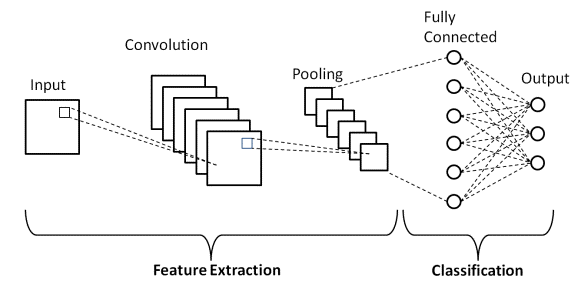
\includegraphics[width=\linewidth]{theorical_foundations/cnn.png}
      \caption{Convolutional Neural Network architecture}
      \label{fig:convolutional_neural_network}
    \end{figure}
    CNN are useful for image classification, object detection, semantic segmentation,
    and many other computer vision tasks\cite{goodfellow2016deep, intelligence2021modern}.
    In the following sections, the fundamentals of the layers that compose a CNN are
    explained.

    \subsubsection{Convolution operation}

      \ti{Convolution operation} is the core operation of a CNN, extracts features
      from the input data by applying a \ti{kernel} to it\cite{goodfellow2016deep, intelligence2021modern}.
      Features like edges, corners, and blobs are extracted from the input data
      by applying a \ti{kernel}, being capable of extracting more complex
      features by stacking multiple \ti{convolutional layers}\cite{goodfellow2016deep, intelligence2021modern}.
      Convolution operation takes two arguments, the first one is often referred as the
      \ti{input} and the second one as the \ti{kernel} or \ti{filter} and outputs
      a \ti{feature map}.
      Convolution operation is defined as follows\cite{goodfellow2016deep}:
      \begin{equation}
        \label{eq:convolution_operation}
        S(i, j) = (I * K)(i, j) = \sum_{m} \sum_{n} I(m, n) K(i - m, j - n)
      \end{equation}
      where $S$ is the \ti{feature map}, $I$ is the \ti{input}, $K$ is the \ti{kernel},
      $i$ and $j$ are the indexes of the \ti{feature map}, and $m$ and $n$ are the
      indexes of the \ti{kernel}.

      The \ti{kernel} is a matrix of weights that is applied to the \ti{input}
      using a sliding window, as shown in figure \ref{fig:convolution_operation}.
      \begin{figure}[htbp]
        \centering
        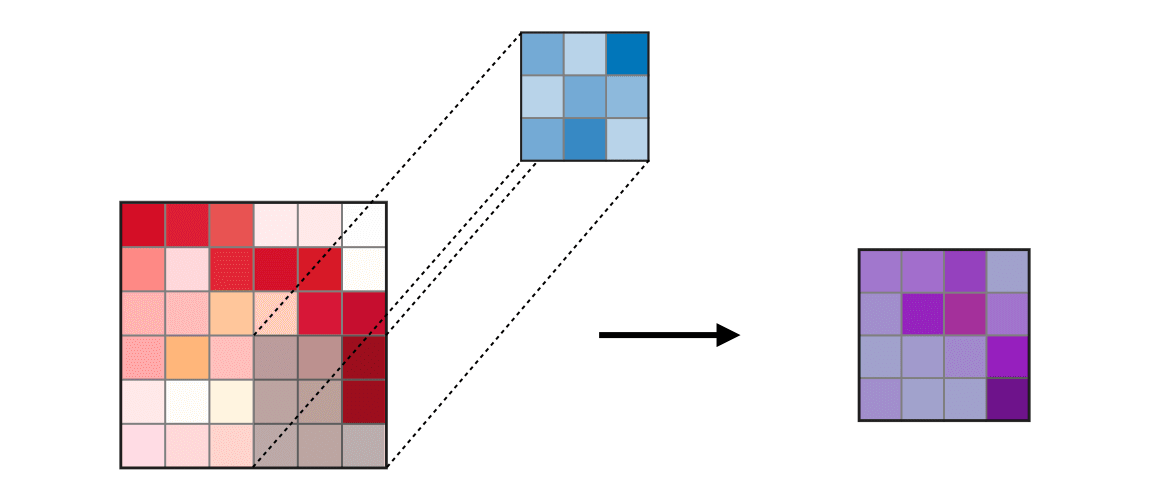
\includegraphics[width=\linewidth]{theorical_foundations/convolution_operation.png}
        \caption{Convolution operation}
        \label{fig:convolution_operation}
      \end{figure}
      Multiply the \ti{kernel} by the \ti{input} using the sliding window and
      sum the results, the new value updates the \ti{feature map} and the sliding
      window moves to the next position. The \ti{kernel} is applied to the whole
      \ti{input} and the result is the \ti{feature map}\cite{goodfellow2016deep, intelligence2021modern}.
      As we can use multiple \ti{kernels} in a convolutional layer, the output
      of a convolutional layer is a \ti{feature map} for each \ti{kernel} used.

    \subsubsection{Pooling}

      \ti{Pooling} is an operation that reduces the size of the \ti{feature map},
      extracting robust and invariant features from it\cite{goodfellow2016deep, intelligence2021modern}.
      Its applied to each \ti{feature map} independently, reducing the size of the
      \ti{feature map} by applying a function to a sliding window
      of the \ti{feature map}, as shown in figure \ref{fig:pooling_operation}.
      \begin{figure}[htbp]
        \centering
        \begin{subfigure}[b]{0.45\linewidth}
          \centering
          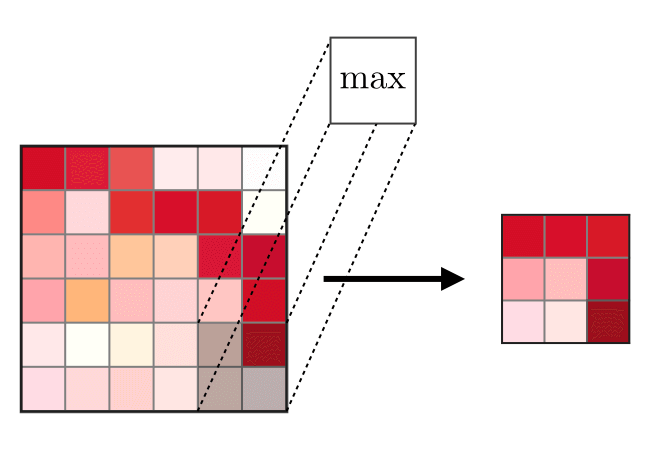
\includegraphics[width=\linewidth]{theorical_foundations/max_pooling.png}
          \caption{Max pooling}
          \label{fig:max_pooling}
        \end{subfigure}
        \begin{subfigure}[b]{0.45\linewidth}
          \centering
          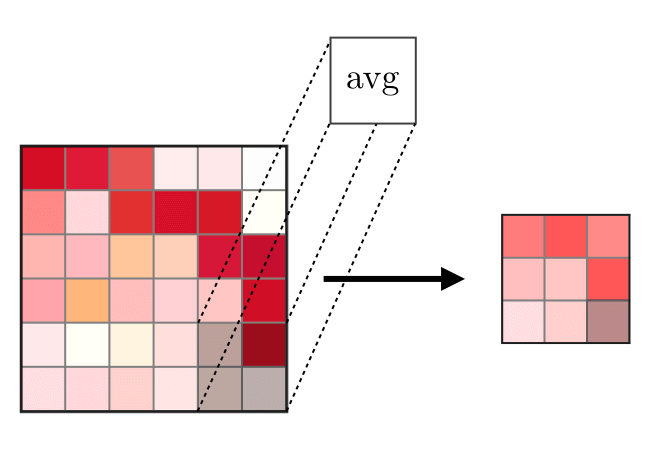
\includegraphics[width=\linewidth]{theorical_foundations/avg_pooling.png}
          \caption{Average pooling}
          \label{fig:avg_pooling}
        \end{subfigure}
        \caption{Pooling operation}
        \label{fig:pooling_operation}
      \end{figure}

      The most common \ti{pooling} operations are \ti{max pooling} and \ti{average pooling},
      where \ti{max pooling} outputs the maximum value of the sliding window and
      \ti{average pooling} outputs the average value of the sliding window\cite{goodfellow2016deep, intelligence2021modern}.
      These pooling functions provides various strategies to downsample feature maps,
      extract invariant features, and reduce spatial dimensions in order to reduce
      the number of parameters and computation in CNN architecture.

    \subsubsection{Fully Connected Layers}

      \ti{Fully connected layers} are used to classify the input data, they are
      composed of a series of neurons that are connected to all the neurons of
      the previous layer, as shown in figure \ref{fig:fully_connected_layer}.
      \begin{figure}[htbp]
        \centering
        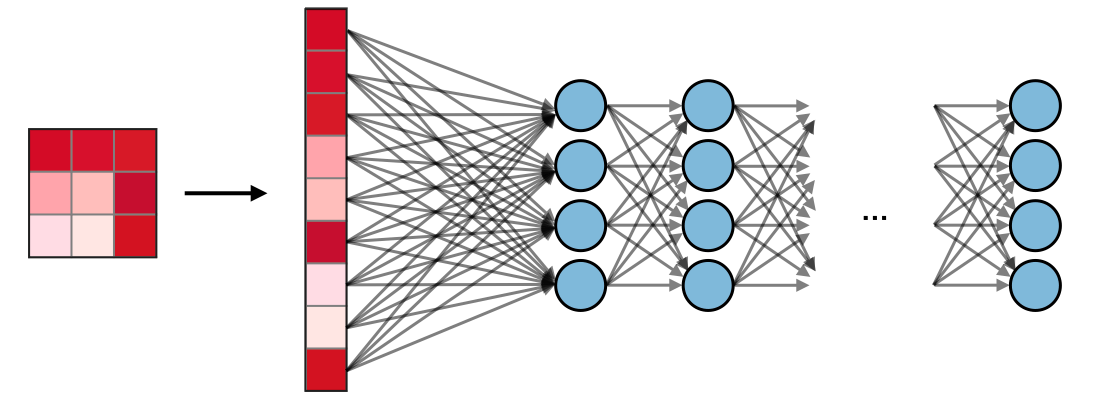
\includegraphics[width=\linewidth]{theorical_foundations/fully_connected.png}
        \caption{Fully connected layer}
        \label{fig:fully_connected_layer}
      \end{figure}
      Typically, the last layer of a CNN is a \ti{fully connected layer} that
      performs the classification of the input data, enables the network to
      learn non-linear combinations of features extracted by the previous layers,
      and outputs a vector of probabilities that represents the probability of
      the input data to belong to each class\cite{goodfellow2016deep, intelligence2021modern}.

    \subsubsection{Activation Functions}

      \ti{Activation functions} are used to introduce non-linearity to the network,
      they are applied to the output of each neuron of a CNN\cite{goodfellow2016deep, intelligence2021modern}.
      The most common \ti{activation functions} are \ti{sigmoid}, \ti{tanh}, and
      \ti{ReLU}, as shown in figure \ref{fig:activation_functions}.
      \begin{figure}[htbp]
        \centering
        \begin{subfigure}[b]{0.30\linewidth}
          \centering
          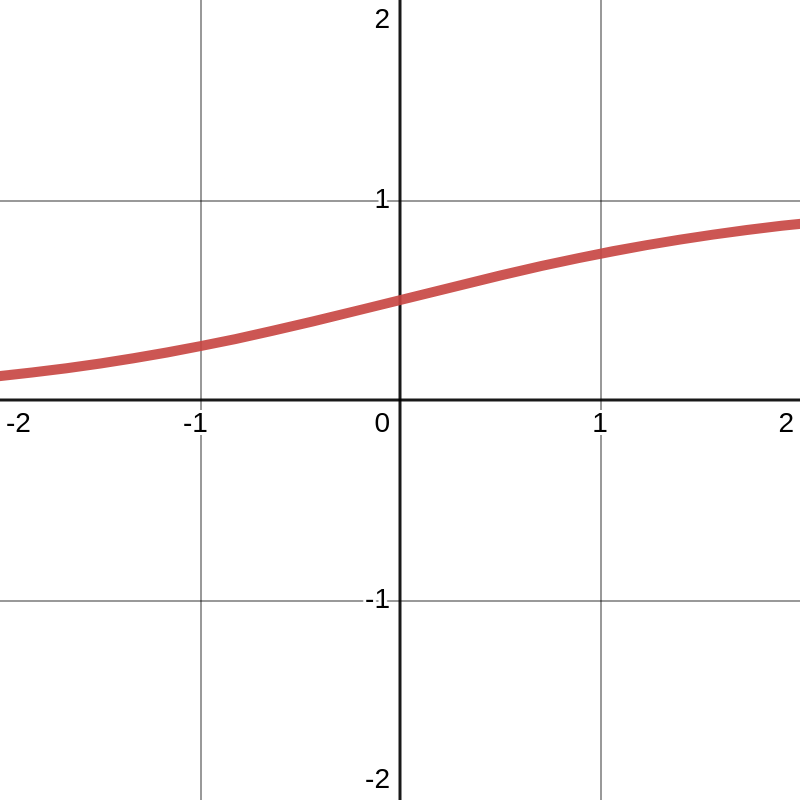
\includegraphics[width=\linewidth]{theorical_foundations/sigmoid.png}
          \caption{Sigmoid}
          \label{fig:sigmoid}
        \end{subfigure}
        \begin{subfigure}[b]{0.30\linewidth}
          \centering
          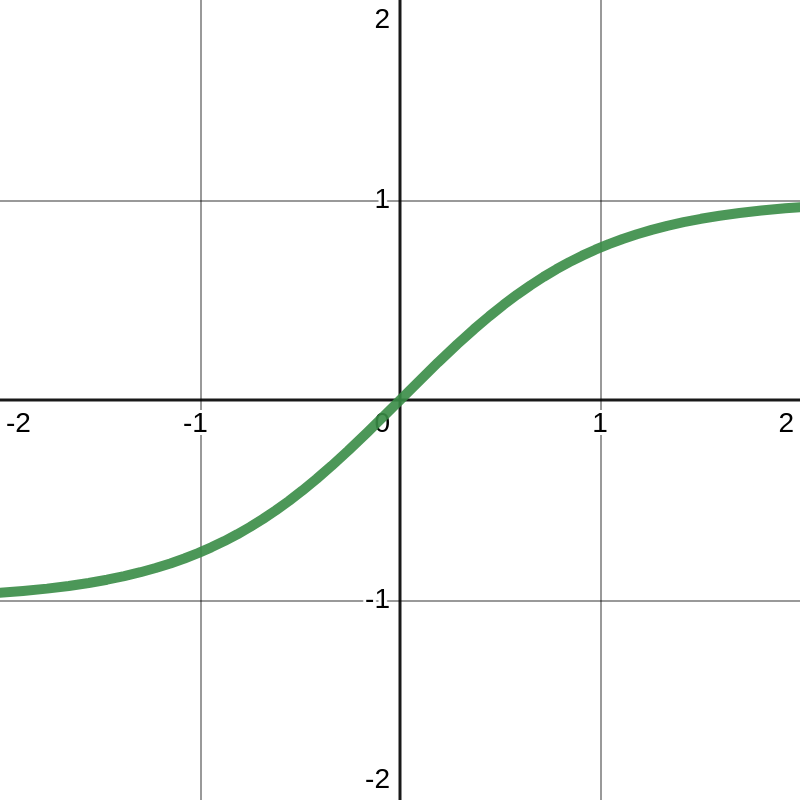
\includegraphics[width=\linewidth]{theorical_foundations/tanh.png}
          \caption{Tanh}
          \label{fig:tanh}
        \end{subfigure}
        \begin{subfigure}[b]{0.30\linewidth}
          \centering
          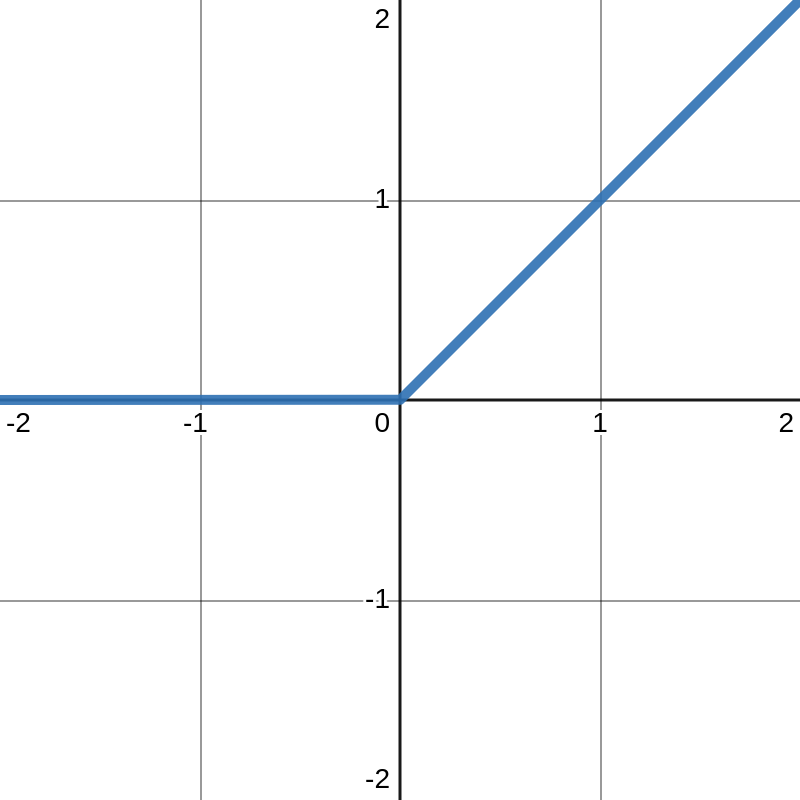
\includegraphics[width=\linewidth]{theorical_foundations/relu.png}
          \caption{ReLU}
          \label{fig:relu}
        \end{subfigure}
        \caption{Activation functions}
        \label{fig:activation_functions}
      \end{figure}

      \tb{Sigmoid activation function} is defined as follows\cite{goodfellow2016deep}:
      \begin{equation}
        \label{eq:sigmoid_activation_function}
        \sigma(x) = \frac{1}{1 + e^{-x}}
      \end{equation}
      where $x$ is the input of the neuron. The output of the \ti{sigmoid activation
      function} is a value between 0 and 1, which is useful for binary classification
      problems\cite{goodfellow2016deep, intelligence2021modern}.

      \tb{Tanh activation function} is defined as follows\cite{goodfellow2016deep}:
      \begin{equation}
        \label{eq:tanh_activation_function}
        \tanh(x) = \frac{e^{x} - e^{-x}}{e^{x} + e^{-x}}
      \end{equation}
      where $x$ is the input of the neuron. The output of the \ti{tanh activation
      function} is a value between -1 and 1, which is useful for classification
      problems\cite{goodfellow2016deep, intelligence2021modern}.

      \tb{ReLU activation function} is defined as follows\cite{goodfellow2016deep}:
      \begin{equation}
        \label{eq:relu_activation_function}
        \text{ReLU}(x) = \max(0, x)
      \end{equation}
      where $x$ is the input of the neuron. The output of the \ti{ReLU activation
      function} is a value between 0 and $\infty$, which is useful for classification
      problems\cite{goodfellow2016deep, intelligence2021modern}.

      \ti{Sigmoid} and \ti{tanh} are used in the past, but \ti{ReLU} is the most
      common \ti{activation function} used nowadays\cite{goodfellow2016deep, intelligence2021modern}.
  
  \subsection{Fundamentals of Transformers}

    \ti{Transformers} are a groundbreaking architecture that has been used in
    many NLP tasks\cite{goodfellow2016deep}. They are based on the \ti{attention}
    mechanism, which is a mechanism that allows the network to focus on the
    relevant parts of the input data\cite{goodfellow2016deep, vaswani2017attention}.
    Transformers are composed of an \ti{encoder} and a \ti{decoder}, as shown
    in figure \ref{fig:transformer_architecture}.
    \begin{figure}[htbp]
      \centering
      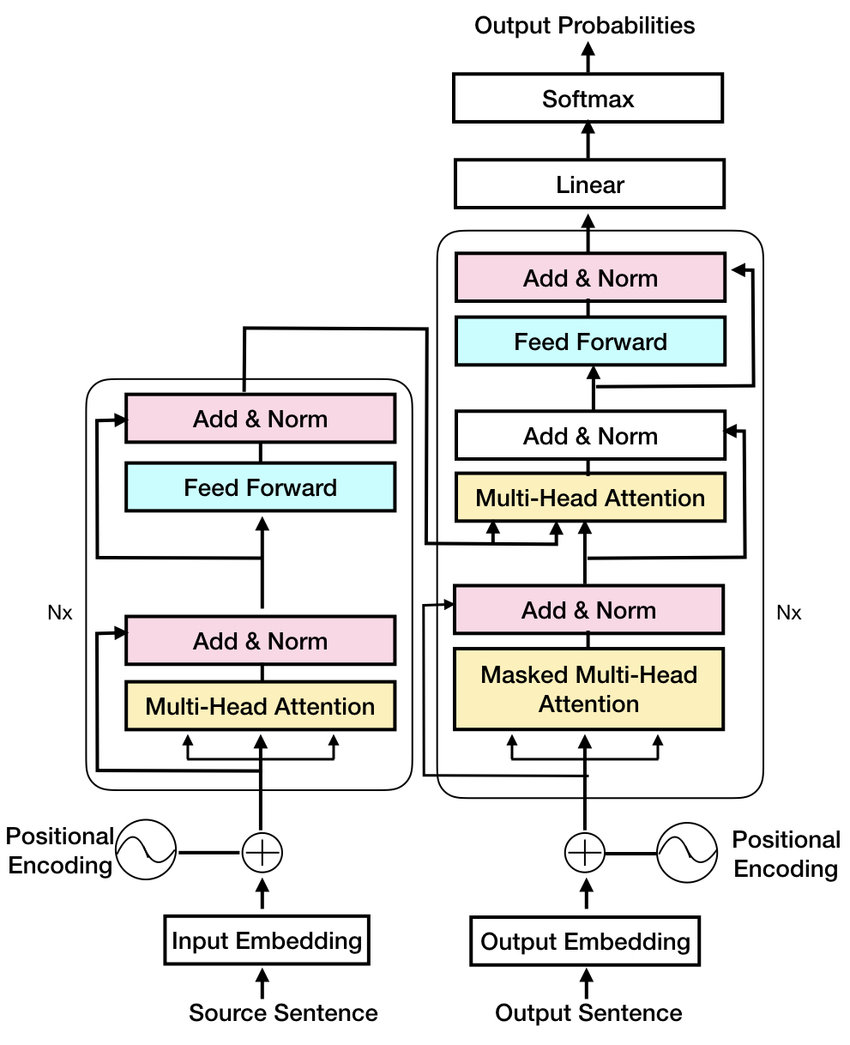
\includegraphics[width=\linewidth]{theorical_foundations/transformer_architecture.png}
      \caption{Transformer architecture\cite{vaswani2017attention}}
      \label{fig:transformer_architecture}
    \end{figure}

    \subsubsection{Encoder}

      \ti{Encoder layer} is composed of two sub-layers: \ti{multi-head attention} and
      \ti{feed-forward network} as seen in \ref{fig:encoder_layer}.
      \begin{figure}[htbp]
        \centering
        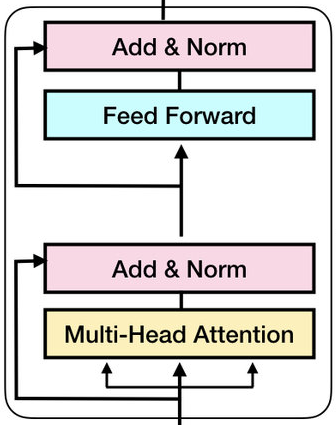
\includegraphics[width=0.50\linewidth]{theorical_foundations/encoder_layer.png}
        \caption{Encoder layer\cite{vaswani2017attention}}
        \label{fig:encoder_layer}
      \end{figure}
      Encoder extracts meaningful features from the input data, tipically
      a sequence of token representations and produces a set of feature vectors
      that capture the semantics and dependencies of the input data\cite{vaswani2017attention}.
      Self-attention mechanism enables the network to attend to the relevant
      parts of the input data, and weight the importance of each token in the
      sequence\cite{vaswani2017attention}. Encoder is composed of a stack of
      \ti{encoder layers} described above, also using residual connections and
      layer normalization as shown in figure \ref{fig:encoder_layer}.

    \subsubsection{Decoder}

      \ti{Decoder layer} is composed of three sub-layers: \ti{masked multi-head attention},
      \ti{multi-head attention}, and \ti{feed-forward network} as seen in \ref{fig:decoder_layer}.
      \begin{figure}[htbp]
        \centering
        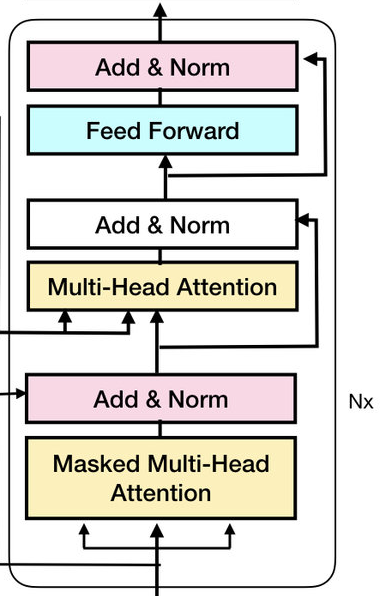
\includegraphics[width=0.50\linewidth]{theorical_foundations/decoder_layer.png}
        \caption{Decoder layer\cite{vaswani2017attention}}
        \label{fig:decoder_layer}
      \end{figure}
      Decoder takes the output of the encoder and produces a sequence of token
      representations that are used to generate the output data\cite{vaswani2017attention}.
      \ti{Masked multi-head attention} is used to prevent the network from attending
      to the future tokens in the sequence\cite{vaswani2017attention}.
      \ti{Multi-head attention} is used to attend to the relevant parts of the
      input data\cite{vaswani2017attention}.
      \ti{Feed-forward network} is used to learn non-linear combinations of features
      extracted by the \ti{multi-head attention} sub-layer\cite{vaswani2017attention}.
      Each \ti{Decoder} is composed of a stack of \ti{decoder layers} described
      above, also using residual connections and layer normalization as shown in
      figure \ref{fig:decoder_layer}.

    Tipically, both \ti{encoder} and \ti{decoder} are composed of 6 layers\cite{vaswani2017attention}.
    Encoder processes the input data and extracts meaningful features from it and decoder
    generates the output data based on the features extracted by the encoder\cite{vaswani2017attention}.
